\documentclass[a4j,twocolumn,10pt]{jsarticle}
%\documentclass{ipsjpapers}
%\makeatletter
%\def\documentstyle#1{}
\pagestyle{empty}
% 画像挿入用パッケージ
\usepackage[dvipdfmx]{graphicx}
\usepackage{url}
%\usepackage{cite}
\usepackage{bm}
\newcommand\figref[1]{\textbf{Figure~\ref{fig:#1}}}
\newcommand\tabref[1]{\textbf{Table~\ref{tab:#1}}}
\usepackage{color}
\usepackage{multirow}
\usepackage{diagbox}
\usepackage{amsmath}



% 巻数,号数などの設定
%\setcounter{巻数}{41}
%\setcounter{号数}{6}
%\setcounter{volpageoffset}{1234}
%\受付{12}{2}{4}
%\採録{12}{5}{11}

% ユーザが定義したマクロなど.
\makeatletter
%\let\@ARRAY\@array \def\@array{\def\<{\inhibitglue}\@ARRAY}
%\def\<{\(\langle\)}
%\def\>{\(\rangle\)}
%\def\|{\verb|}
%\def\Underline{\setbox0\hbox\input{topic_presentation.tex}
\bgroup\let\\\endUnderline
%\def\endUnderline{\vphantom{y}\egroup\smash{\underline{\box0}}\\}
%\def\LATEX{\iLATEX\Large}
%\def\LATEx{\iLATEX\normalsize}
%\def\LATex{\iLATEX\small}
%\def\iLATEX#1{L\kern-.36em\raise.3ex\hbox{#1\bf A}\kern-.15em
%    T\kern-.1667em\lower.7ex\hbox{E}\kern-.125emX}
%\def\LATEXe{\ifx\LaTeXe\undefined \LaTeX 2e\else\LaTeXe\fi}
%\def\LATExe{\ifx\LaTeXe\undefined \iLATEX\scriptsize 2e\else\LaTeXe\fi}
%\def\Quote{\list{}{}\item[]}
%\let\endQuote\endlist
%\def\TT{\if@LaTeX@e\tt\fi}
%\def\CS#1{\if@LaTeX@e\tt\expandafter\string\csname#1\endcsname\else
%	$\backslash$#1\fi}

\def\section{\@startsection{section}{1}{\z@}{3ex plus .2ex minus .2ex}%
			{.5ex plus .2ex minus .2ex}{\large\bfseries}}
\def\thesection{\arabic{section}.}
\def\subsection{\@startsection{subsection}{1}{\z@}{3ex plus .2ex minus .2ex}%
			{.2ex plus .2ex minus .2ex}{\normalsize\bfseries}}
\def\thesubsection{\arabic{section}.\arabic{subsection}}
\def\subsubsection{\@startsection{subsubsection}{1}{\z@}{2ex plus .2ex minus .2ex}%
			{.2ex plus .2ex minus .2ex}{\normalsize\bfseries}}
\def\thesubsubsection{\arabic{section}.\arabic{subsection}.\arabic{subsubsection}}


%\def\thefootnote{\fnsymbol{footnote}}
\makeatother

\def\baselinestretch{0.850}

\setlength{\textheight}{24.5cm}%297-30-27 - 5
\setlength{\textwidth}{17.0cm}%210-18-18 - 10
%\setlength{\headheight}{0.0in}
\setlength{\headsep}{-0.3in}
\setlength{\oddsidemargin}{-.4cm}%+3
%\setlength{\evensidemargin}{-.9cm}%+3
\setlength{\columnsep}{7mm}

%文章途中に挿入された図表の余白
%\setlength\intextsep{12pt plus 2pt minus 2pt}
%ページ上部の図と図の余白
%\setlength{\floatsep}{9pt plus 2pt minus 0pt}
%ページ上部の図と本文の余白
%\setlength\textfloatsep{20pt plus 2pt minus 4pt}





\renewcommand{\thefootnote}{\arabic{footnote}}

%\checklines	% 行送りを確認する時に使用

\begin{document}%{
\pagestyle{plain}
%\renewcommand{\thepage}{-- \arabic{page} --}
\twocolumn[%
%\begin{center}
\vspace{-0.8cm}
\title{\Large 
ディスプレイを用いて光電脈波センサに任意の脈波を計測させる手法\\
\vspace{.9ex}
}

\author{藤井敦寛 \vspace{0.3cm} \\
{情報理工学研究科 計算機科学コース 知的インタラクティブシステム研究室}\\
{6611200054-3}\\
{atsuhiro.fujii@iis.ise.ritsumei.ac.jp}}

\date{\hfill}

\maketitle
\thispagestyle{empty}
\pagestyle{empty}
\vspace{-1.5cm}

\vspace{1.0cm}
]




%\setcounter{footnote}{2}
%\footnotetext{http://www.amazon.com/}

\section{研究の背景と目的}
\label{introduction}
健康管理への意識の高まりから,自身の生体情報を記録するウェアラブルデバイスが広く普及している.記録する生体情報は活動量や呼吸数,体温などさまざまな情報があり,心拍数もそのひとつである.心拍数を取得するために用いられる脈波センサは,緑色のLEDを皮膚に照射して,血管を通して反射した光の変化から脈波を計測する光電式容積脈波記録法(PPG)と呼ばれる方式のものが一般的であり,市販のスマートウォッチに導入されている.スマートウォッチのセンサから取得できる心拍データを用いて疲労度を検出する手法を今井ら\cite{fatigue_detection}が提案している.そのほか,Hanら\cite{arrhythmia_detection}はスマートウォッチから取得された脈波データから心房期外収縮(PAC)および,心室性期外収縮(PVC)を検出する手法を提案している.このように,脈波センサから得られるデータを使用した研究は盛んである.

しかしながら,義手やロボットアームなど人工的な身体には血流が存在しないためスマートウォッチを生身の身体と同様に手首に装着して生体情報を計測することはできない.通話やメッセージ,時計などのスマートウォッチの機能や加速度センサやGPSなどのセンサは人工的な身体でも利用できるが,生体情報の計測はできない.このように,人工的な身体において生身の身体で利用できていたインタフェース,デザイン,プロトコルが利用できない問題がある.この問題を解決するには,現状では追加のセンサを計測可能な身体部位に装着して,何からの通信手段を用いてセンサデータを収集する必要がある.しかし,仮に収集したとしても,スマートウォッチが提供するアプリにデータを与えてサービスを利用することはハードルが高いため,スマートウォッチに搭載されているセンサに計測させたい.しかし,計測可能部位にスマートウォッチを装着すると,本来のスマートウォッチとしての機能(時計やディスプレイ表示,タッチ操作)が利用できなくなるため,スマートウォッチ本来の使用形態である手首に装着して脈拍などの生体情報を計測できるようにすることが望ましい.
\par

本研究では,ディスプレイを用いて脈波センサに脈波データを計測させる手法を検討する.ディスプレイの表示を変化させることで任意の脈波データを脈波センサに読み取らせることができれば,義手やロボットアームなどの人工的な身体にスマートウォッチを装着する場合でも,身体と義手の接合部などで計測された脈波を入力することで,その値をスマートウォッチに読み取らせることができ,スマートウォッチが提供する機能を生身の身体と同様に利用できる.また,人工的な身体にディスプレイを搭載するのみでスマートウォッチには手を加えないため,市販のスマートウォッチをそのまま利用できる.このほか,遠隔地のロボットアバタに適用すれば,操作者の生体情報をアバタの身体でも計測できるようになる.本稿では,ディスプレイによる脈波生成の予備段階として,あらかじめ収集された実際の脈波データを参考にして,ディスプレイの色調を変化させることで,任意の心拍数を計測させる手法を提案する.ディスプレイを用いて脈波センサに脈波データを計測させることができるかを確認し,提案手法の有効性を明らかにする.
\par





\section{提案手法}
\label{sec:method}


\subsection{概要}
\label{subsec:overview}
提案手法は任意の心拍数を設定すると,ディスプレイの表示が変化し,ディスプレイ上に装着したスマートウォッチに指定された心拍数を計測させる.提案手法の処理の流れを\figref{method}に示す.はじめに,身体と義手の接合部に別途PPGセンサを装着し,得られた脈波データから心拍数を算出する.これを目標心拍数$H_{target}$とし,目標心拍数に応じてディスプレイの明暗を変化させる.そして,ディスプレイ上に装着されたスマートウォッチは目標心拍数と同じ数値の心拍数を計測する.

\begin{figure}[!t]
  \centering
  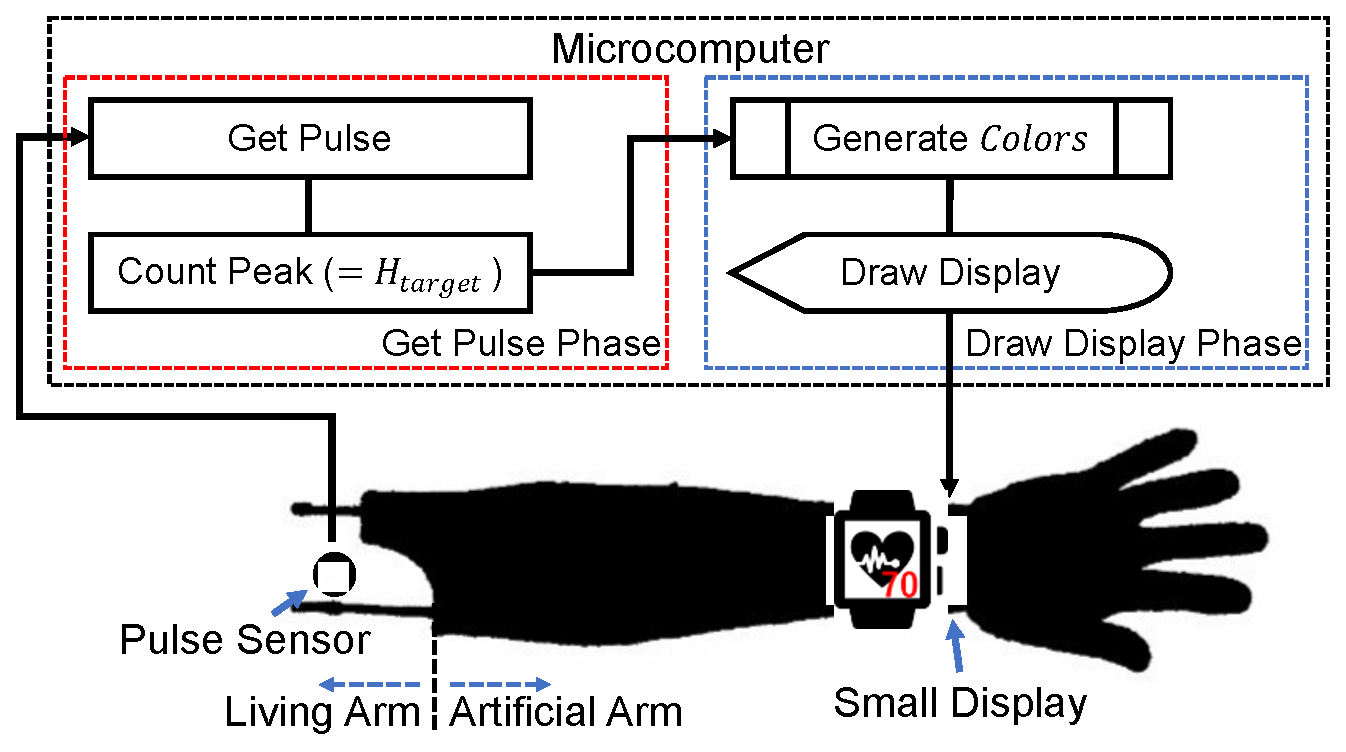
\includegraphics[width=0.8\linewidth]{figures/method.eps}
  \caption{提案手法の概要}
  \label{fig:method}
\end{figure}


\subsection{ディスプレイの制御}
スマートウォッチが計測する心拍数が$H_{target}$となるように,ディスプレイの明暗を制御する.事前に,1回の脈拍をスマートウォッチに検出させることができるディスプレイの明暗の変化のグレースケールデータ列$Colors$を用意する.ヒューリスティックに探索した事前調査から$Colors$は以下の流れで生成した.
\begin{equation*}
  Colors[i]=\min\left(\sin\left(\frac{2\pi i}{L}\right)+1,1\right)*SCALE+BASE
\end{equation*}
1分間で$Colors$が$H_{target}$回だけ再生されるように,$T=\frac{60}{L * H_{target}}$[s]ごとに$Colors$の値を1つずつ描画する.



\section{評価}
\label{sec:evaluation}


\subsection{実験環境}
スマートウォッチにはTicWatch Pro WF12106(Mobvoi社製)を使用し,ディスプレイはプログラムの実行に使用するノートPCであるLegion 7 15IMH05(Lenovo社製)の内蔵ディスプレイ(以下Display A)とマイクロコンピュータであるRaspberry Pi向けに設計された小型の3.5インチディスプレイ(OSOYOO社製)(以下Display B)を使用した.プログラムを実行するノートPCとDisplay Bの接続にはHDMIを使用した.目標心拍数を成人の平均心拍数である60回から100回\footnote{\url{https://www.heart.org/en/healthy-living/fitness/fitness-basics/target-heart-rates}}まで5刻みで増加させながらデータを取得していき,100回に達すると再度60回から取得を繰り返す流れを3セット行う.

\begin{figure}[!t]
  \centering
  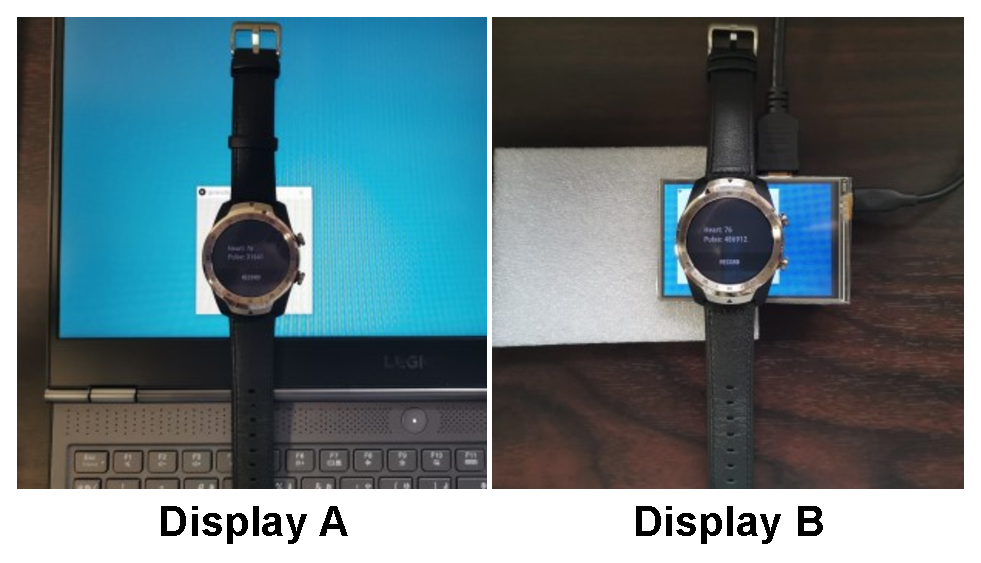
\includegraphics[width=0.8\linewidth]{figures/smartwatches.eps}
  \caption{評価実験での心拍数の取得方法}
  \label{fig:smartwatches}
\end{figure}


\subsection{結果と考察}
設定した目標心拍数とスマートウォッチで取得された心拍数の誤差を\tabref{heartrate}に示す.この結果は3セットの平均値である.0は目標心拍数と一致していることを示し,マイナスは回数が不足していることを示す.また,``Average''はディスプレイごとの誤差の平均値である.結果より,成人の平均心拍数である60回$\sim$100回において,目標心拍数より0$\sim$-3回以内の誤差でスマートウォッチに心拍数を入力できていることが確認できた.平均値ではあるが,目標心拍数を70回としたとき,Display Bを使用してスマートウォッチに心拍数を正しく入力できた.全体の平均としては目標心拍数よりDisplay Aでは1.8回少なく,Display Bでは1.6回少ないという結果となった.

\begin{table}[!t]
  \centering
  \caption{設定した目標心拍数とスマートウォッチで取得された心拍数の誤差}
  \begin{tabular}{c|c|c} \hline\hline
    目標心拍数 & Display A & Display B \\ \hline
    60 & -1.0 & -1.0 \\
    65 & -1.3 & -1.3 \\
    70 & -1.0 & 0.0 \\
    75 & -2.0 & -1.7 \\
    80 & -2.0 & -2.0 \\
    85 & -2.0 & -2.3 \\
    90 & -2.0 & -2.0 \\
    95 & -2.0 & -1.7 \\
    100 & -2.7 & -2.3 \\ \hline
    Average & -1.8 & -1.6 \\ \hline
  \end{tabular}
  \label{tab:heartrate}
\end{table}



\section{まとめ}
\label{sec:conclude}
本研究では,ディスプレイを用いて光電脈波センサに任意の心拍数を計測させる手法を提案した.ディスプレイ描画プログラムおよび,スマートウォッチアプリケーションを実装し,スマートウォッチとディスプレイ2台を使用して,提案手法の効果を確認するための評価実験を行った.その結果,入力した目標心拍数と実際にスマートウォッチで取得された心拍数の誤差が全体で-3回以内だった.ディスプレイごとの平均はDisplay Aで-1.8回,Display Bで-1.6回という結果であり,高い精度で心拍数が再現できた.\par

今後はディスプレイを用いることで,身体部位から取得された実際の脈波データと同様の脈波データをウェアラブルデバイスに計測させる機構を実装する.そのためには,自動でディスプレイの色調を決定していく必要があるため,適切な生成モデルを設計していく.また,身体部位への装着を想定し,デバイスの小型化を検討していく.



\bibliography{references}
\bibliographystyle{junsrt}

\end{document}
